\begin{chapter-bib}{Google Maps}
  System Design Interview 2とLeetCodeのどちらの模範回答もユーザーの位置を表示する機能と目的地までの案内の機能を提供するサービスが分かれている\cite{sdi2,lc-googlemaps}。
  図\ref{fig:sdi2-googlemaps}のActive UsersやPersonalization DBなどの一部のDBについては、使うべきDBの種類が解説\cite{sdi2}に記載されてない。
  Cassandraの削除は遅い\cite{cassandra-delete}ので、Active Usersなど一時的なデータの格納には向かないと思われる。 
  \begin{figure}
   
    \centering
    \includegraphics[width=\textwidth,keepaspectratio]{build/googlemaps.png} 
    \caption{System Design Interview 2の模範回答}
    \label{fig:sdi2-googlemaps}
  \end{figure}
  全ユーザのモバイルアプリケーションを開発者の指定したタイミイングで一斉にアップグレードすることはできないので、後方互換性を守りにくい機能はモバイルアプリケーションではなくバックエンドに置かねばならない\cite{sdi2}。
  
  \section{LeetCode}
  解答は、ユーザの位置を特定する機能とユーザに道案内を提示する機能に対して個別のアーキテクチャ図を提示する\cite{lc-googlemaps}。
  ユーザの位置情報からマップを更新する。
  Spark Streaming Serviceは、新しいストリーミングサービスに置き変わった\cite{spark-streaming}。
  以下の機能要件は、二点間を移動中に距離とETAを随時通知することであり、ユーザが明示的にリクエストを移動中に送るだけではない。
  Google Mapは地図をcanvas要素で描画する。
  \begin{quote}
    Find distance and ETA while travelling between 2 points.
  \end{quote}
  
  \subsection{User Location Information}
  \begin{description}[labelsep=10pt]
  \item[Websocket Handler] ゲートウェイの役割。スケールアウトする。
  \item[Websocket Manager] デバイスがどのWebsocket Handlerと通信しているかを記録する。
  \item[Location Service] ユーザの位置情報を管理する。
  \item[Map Update Service] 新しい道などの地理的な変化を通知する。
  \item[Traffic Update Service] 移動速度の変化を通知する。
  \item[Graph Processing Service] グラフを更新する。
  \end{description}
  \subsubsection{User Navigation Flow}
  \begin{description}[labelsep=10pt]
  \item[Area Search Service] 現在値を緯度経度に変換する。
  \item[Navigation Tracking Service] ユーザが移動中に道案内を通知する。
  \item[Maps Service] ユーザからの道案内のリクエストを受けつける。
  \item[Historical data service] 過去のETAを蓄積し、最新のETAを計算できないときに、代替としてETAを提供する。
  \item[Segments]
  \end{description}
  \subsubsection{自分の解答}
  \href{https://docs.google.com/drawings/d/1w_a6eJVLqFsHHtm0dchQxM1NNOsW16ENjF7n_MRv6OE/edit}{編集中}
  \begin{figure}[!ht]
    \centering
    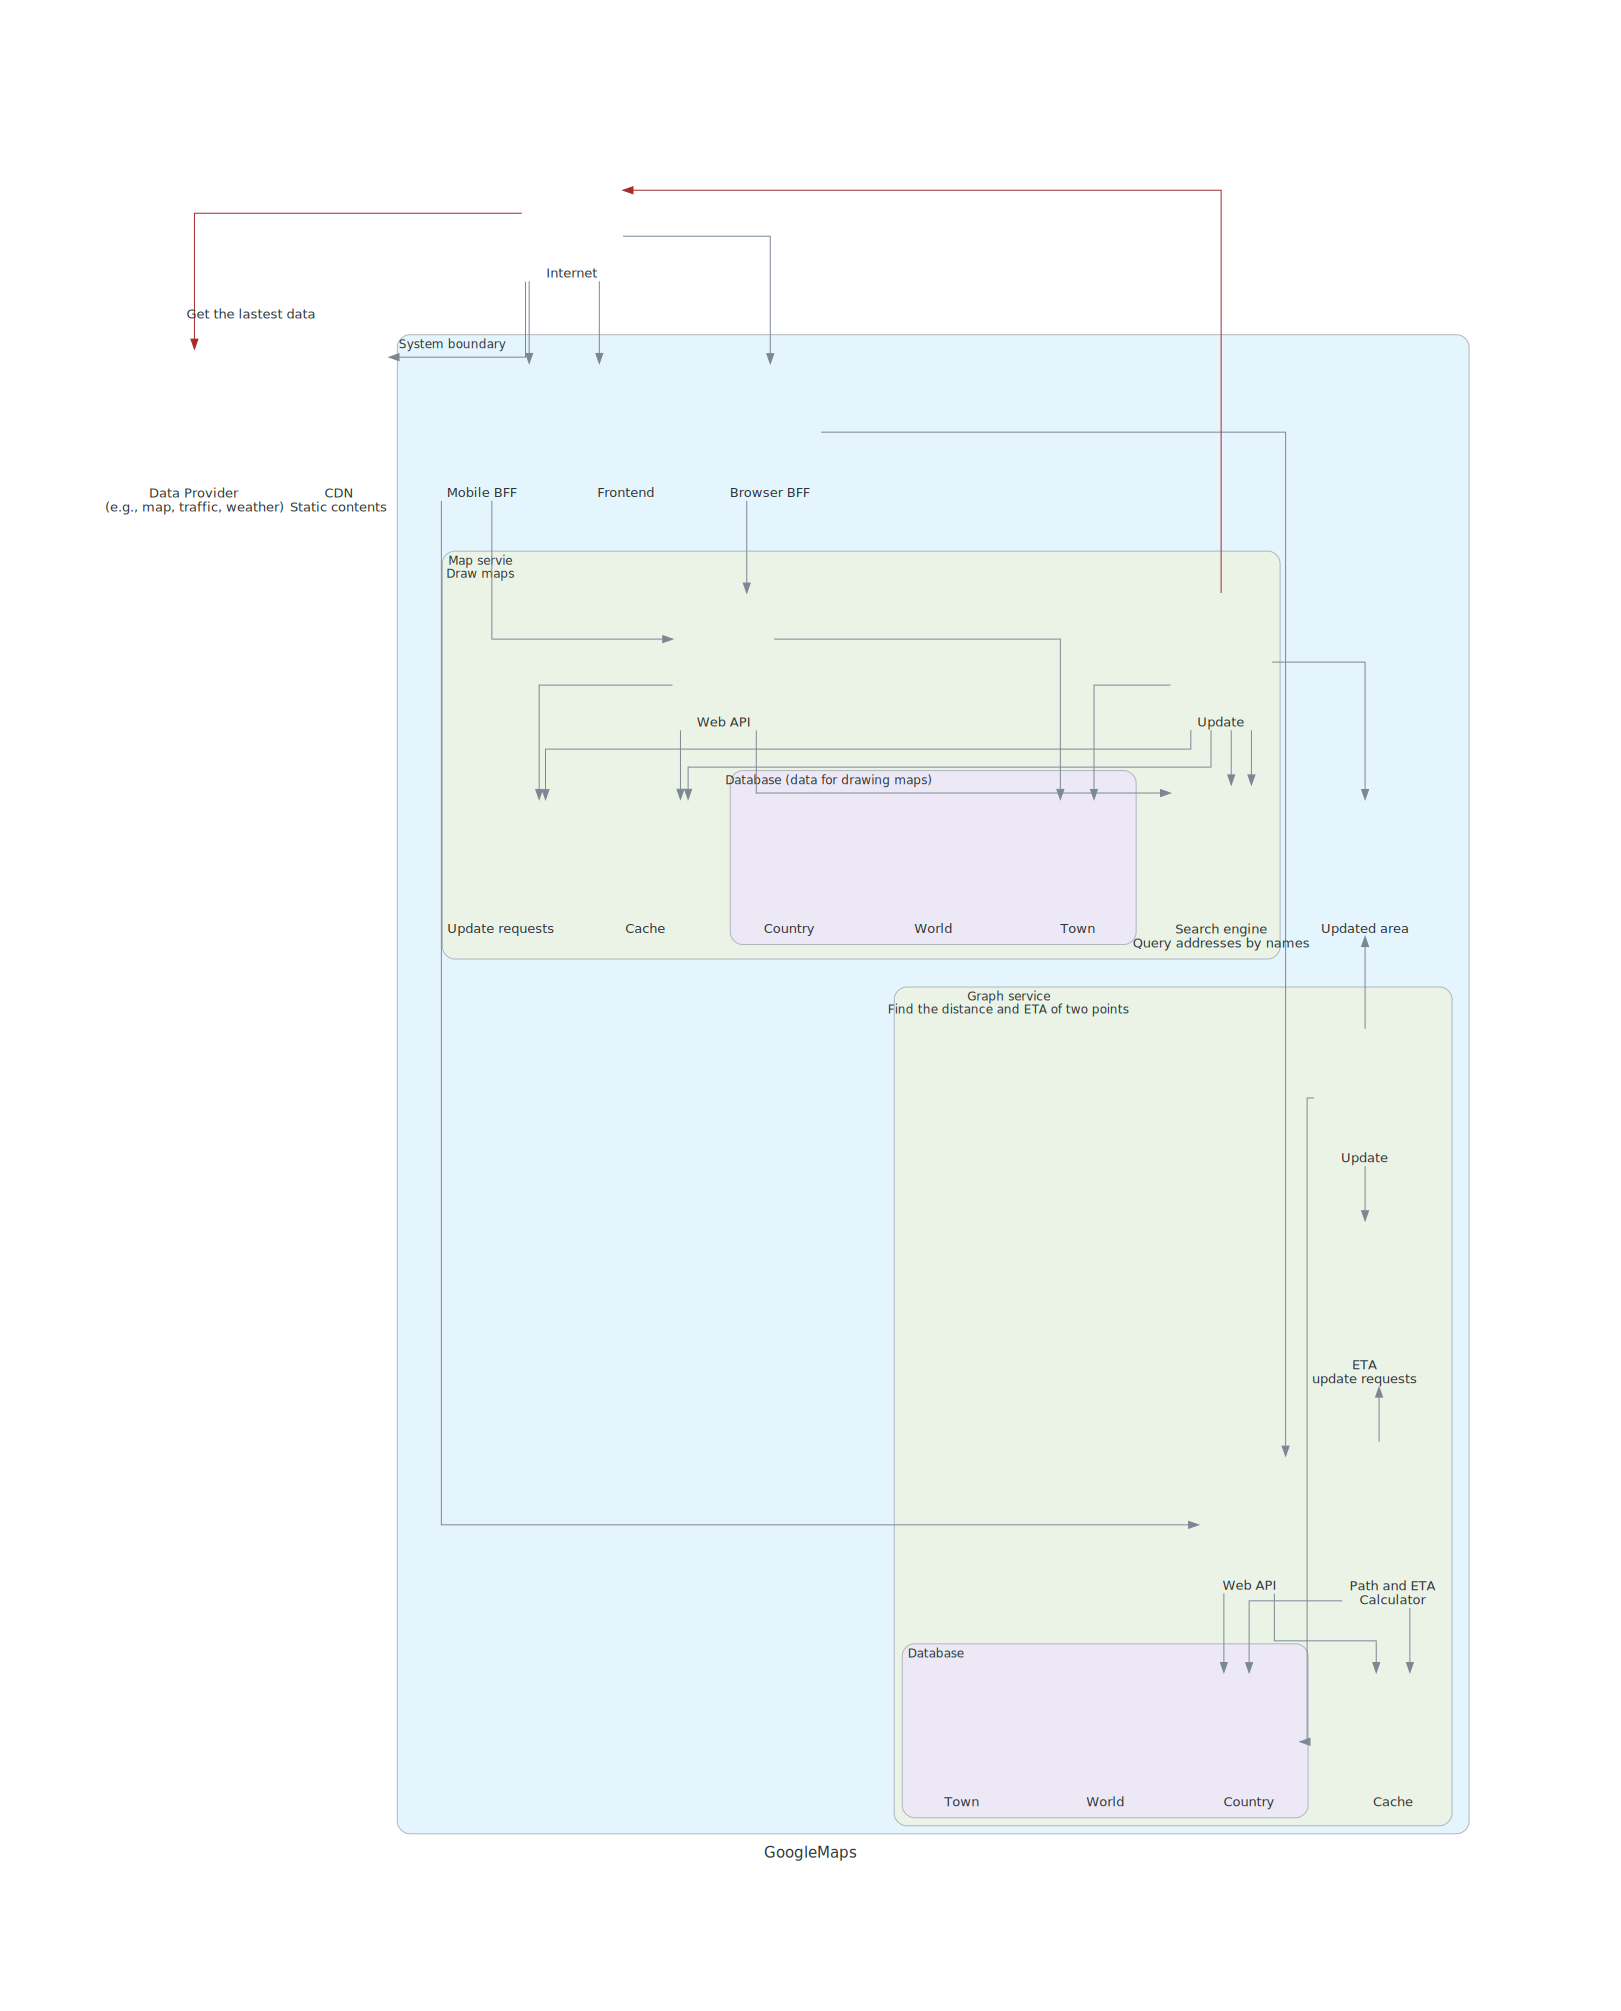
\includegraphics[keepaspectratio, scale=0.20]{build/googlemaps/leetcode.png} 
    \caption{Googlemapsの答案}
    \label{fig:lc-googlemaps}
  \end{figure}
\end{chapter-bib}